\documentclass{beamer}	
\mode<presentation>
 
\usepackage{pdfpages}
\usepackage{fancyvrb}
\usepackage{chemarr}

\usepackage{amsmath}		%% mathematics typesetting
\usepackage{amssymb}
 
\usepackage{epigraph}   %% nice setting of quotations

\usepackage{tabularx} %% allows to use row colours in tables

\usepackage{ulem}

\usepackage{booktabs}

\usepackage{siunitx} %% tpyeset SI units

\usepackage{CJKutf8} %% typeset Chinese characters

\usepackage{pdfpages}%% include pdfs

\usepackage{graphicx}
\usepackage{animate} %% show animated gifs

\DeclareMathAlphabet{\mathcalligra}{T1}{calligra}{m}{n}




% Color and Theme. Can be changed. However, this one's quite nice.
\usetheme{Madrid}
\setbeamertemplate{page number in head/foot}{}

\definecolor{theme}{rgb}{0.84,0,0.21}
\usecolortheme[named=theme]{structure}


% \beamertemplatenavigationsymbolsempty

\begin{document}




%%%%%%%%%%%%%%%%%%%%%%%%%%%%%%%%%%%%%%%%%%%%%%%%%%
%%%%%%%%%%%%%%%%%%%%%%%%%%%%%%%%%%%%%%%%%%%%%%%%%%
%%%%%%%%%%%%%%%%%%%%%%%%%%%%%%%%%%%%%%%%%%%%%%%%%%



\begin{frame}{M11.10 Hormone und Regelkreise}
%% Hormone

%% Einteilung von Hormonen: Chemische Eigenschaften, Wirkungsort, Gewebe der Bildung, Wirkungsweise
%% Regelkreise

\begin{columns}[c]

\begin{column}{5cm}

\begin{block}{nach chemischen Eigenschaften}

 \textbf{Aminosäuren./Peptidderivate}: \\
 Wasserlöslich (außer T3/T4) \\
 Wirken über metabotrope Rezeptoren in der Zellmembran  \\
 Wirken schnell
 
\textbf{Steroidhormone}: \\
Fettlöslich \\
Brauchen Transportproteine \\
Wirken im Inneren der Zelle \\
Wirken langsam \\


\end{block}

\begin{block}{nach chemischen Eigenschaften}
Nach Wirkungsort: parakrin, autokrin, endokrin
\end{block}



\end{column}


\begin{column}{5cm}

\begin{block}{nach Bildungsort}
Glanduläre Hormone (Drüse) \\
Gewebshormone
\end{block}

\pause

\begin{center}
    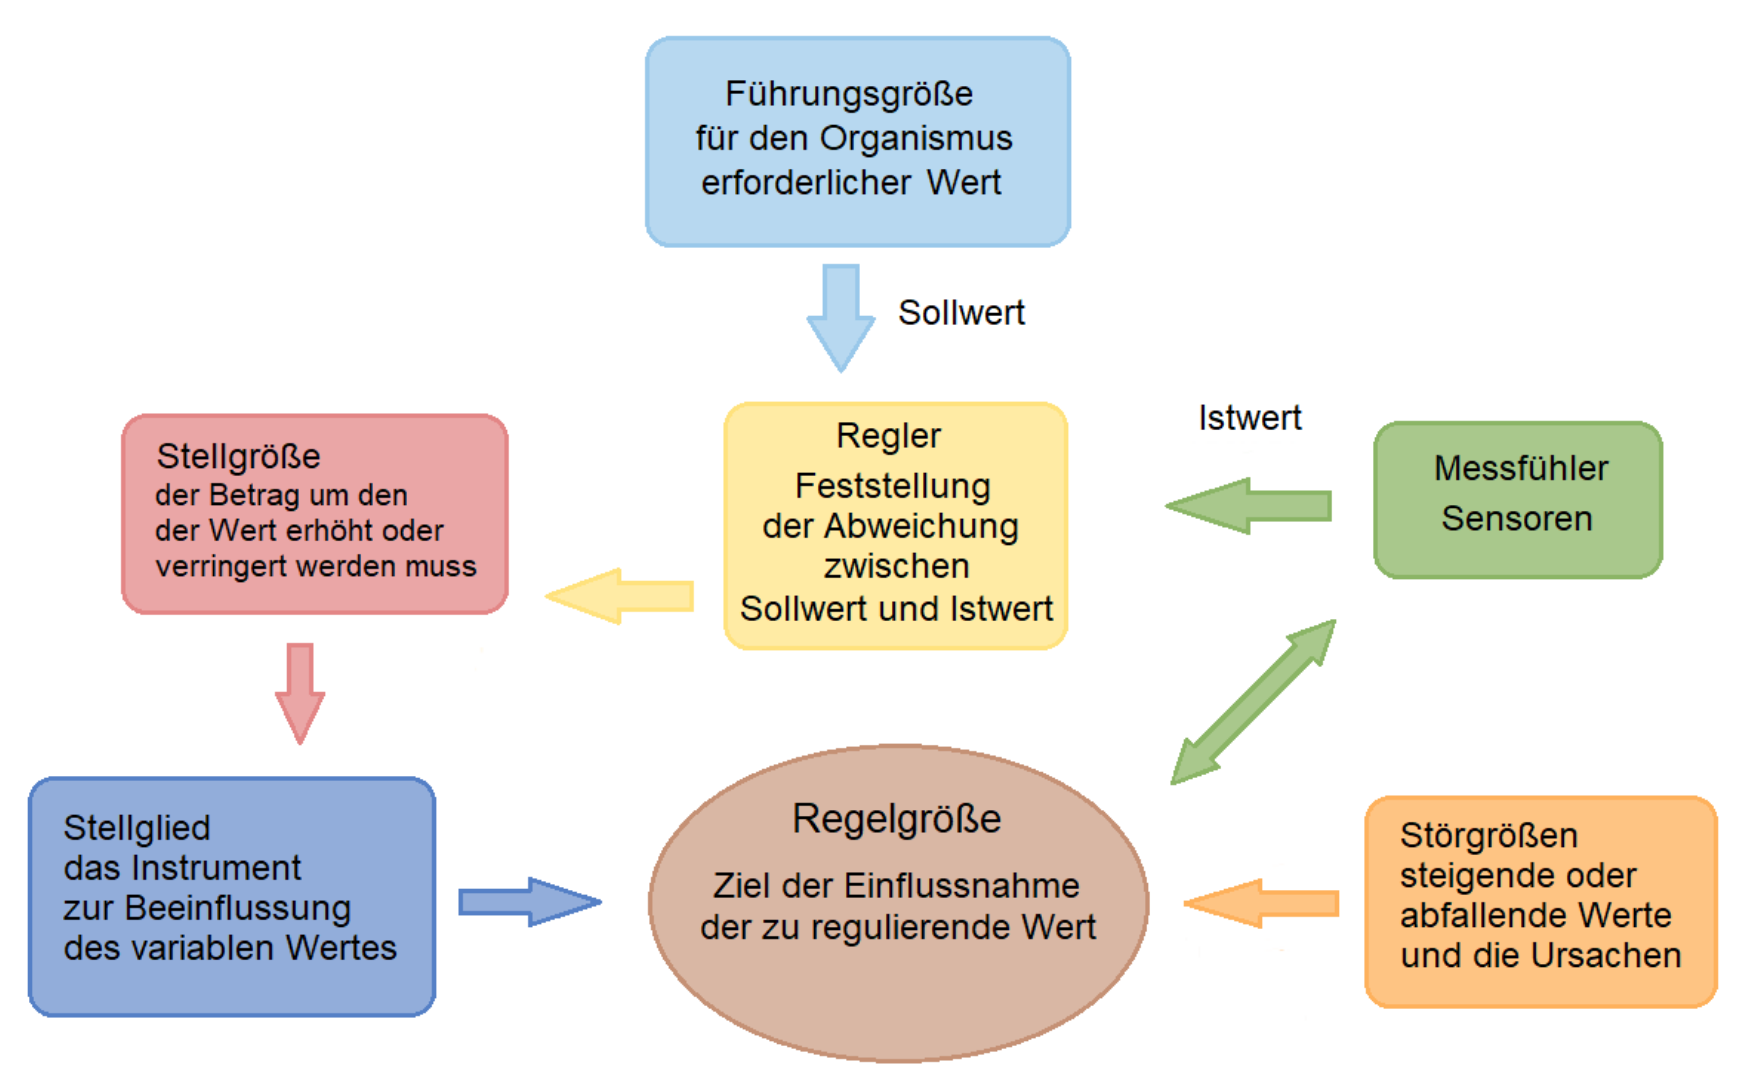
\includegraphics[width=\textwidth]{regelkreis.png}
\end{center}

\end{column}


\end{columns}

    
\end{frame}


%% Hypothalamus Hypophyse allgemein
\begin{frame}{M11.10 Hormone und Regelkreise}

\end{frame}




%% Thyreotropin releasong hormone: 321
%% Cushing Syndrom: 171

%%%%%%%%%%%%%%%%%%%%%%%%%%%%%%%%%%%%%%%%%%%%%%%%%%
%%%%%%%%%%%%%%%%%%%%%%%%%%%%%%%%%%%%%%%%%%%%%%%%%%
%%%%%%%%%%%%%%%%%%%%%%%%%%%%%%%%%%%%%%%%%%%%%%%%%%


% Sexualentwicklung und Reproduktionsphysiologie I:

%% Geschlechtsspezifische Hormone: Chemie, GnRH, LH/FSH, Progesteron/Testosteron/Östrogen
%% Frühe Sexualentwicklung

\begin{frame}{M11.10 Sexualentwicklung und Reproduktionsphysiologie I}

\begin{columns}[c]

\begin{column}{5cm}

\begin{center}
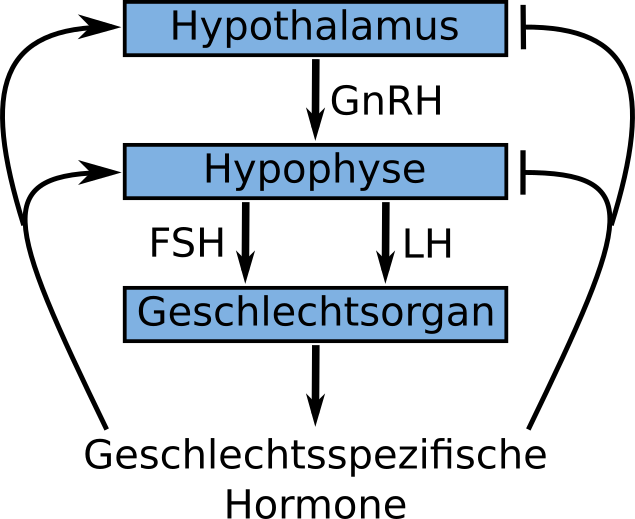
\includegraphics[width=0.7\textwidth]{geschlechtshormone_achse.png}
\end{center}

\pause

\begin{center}
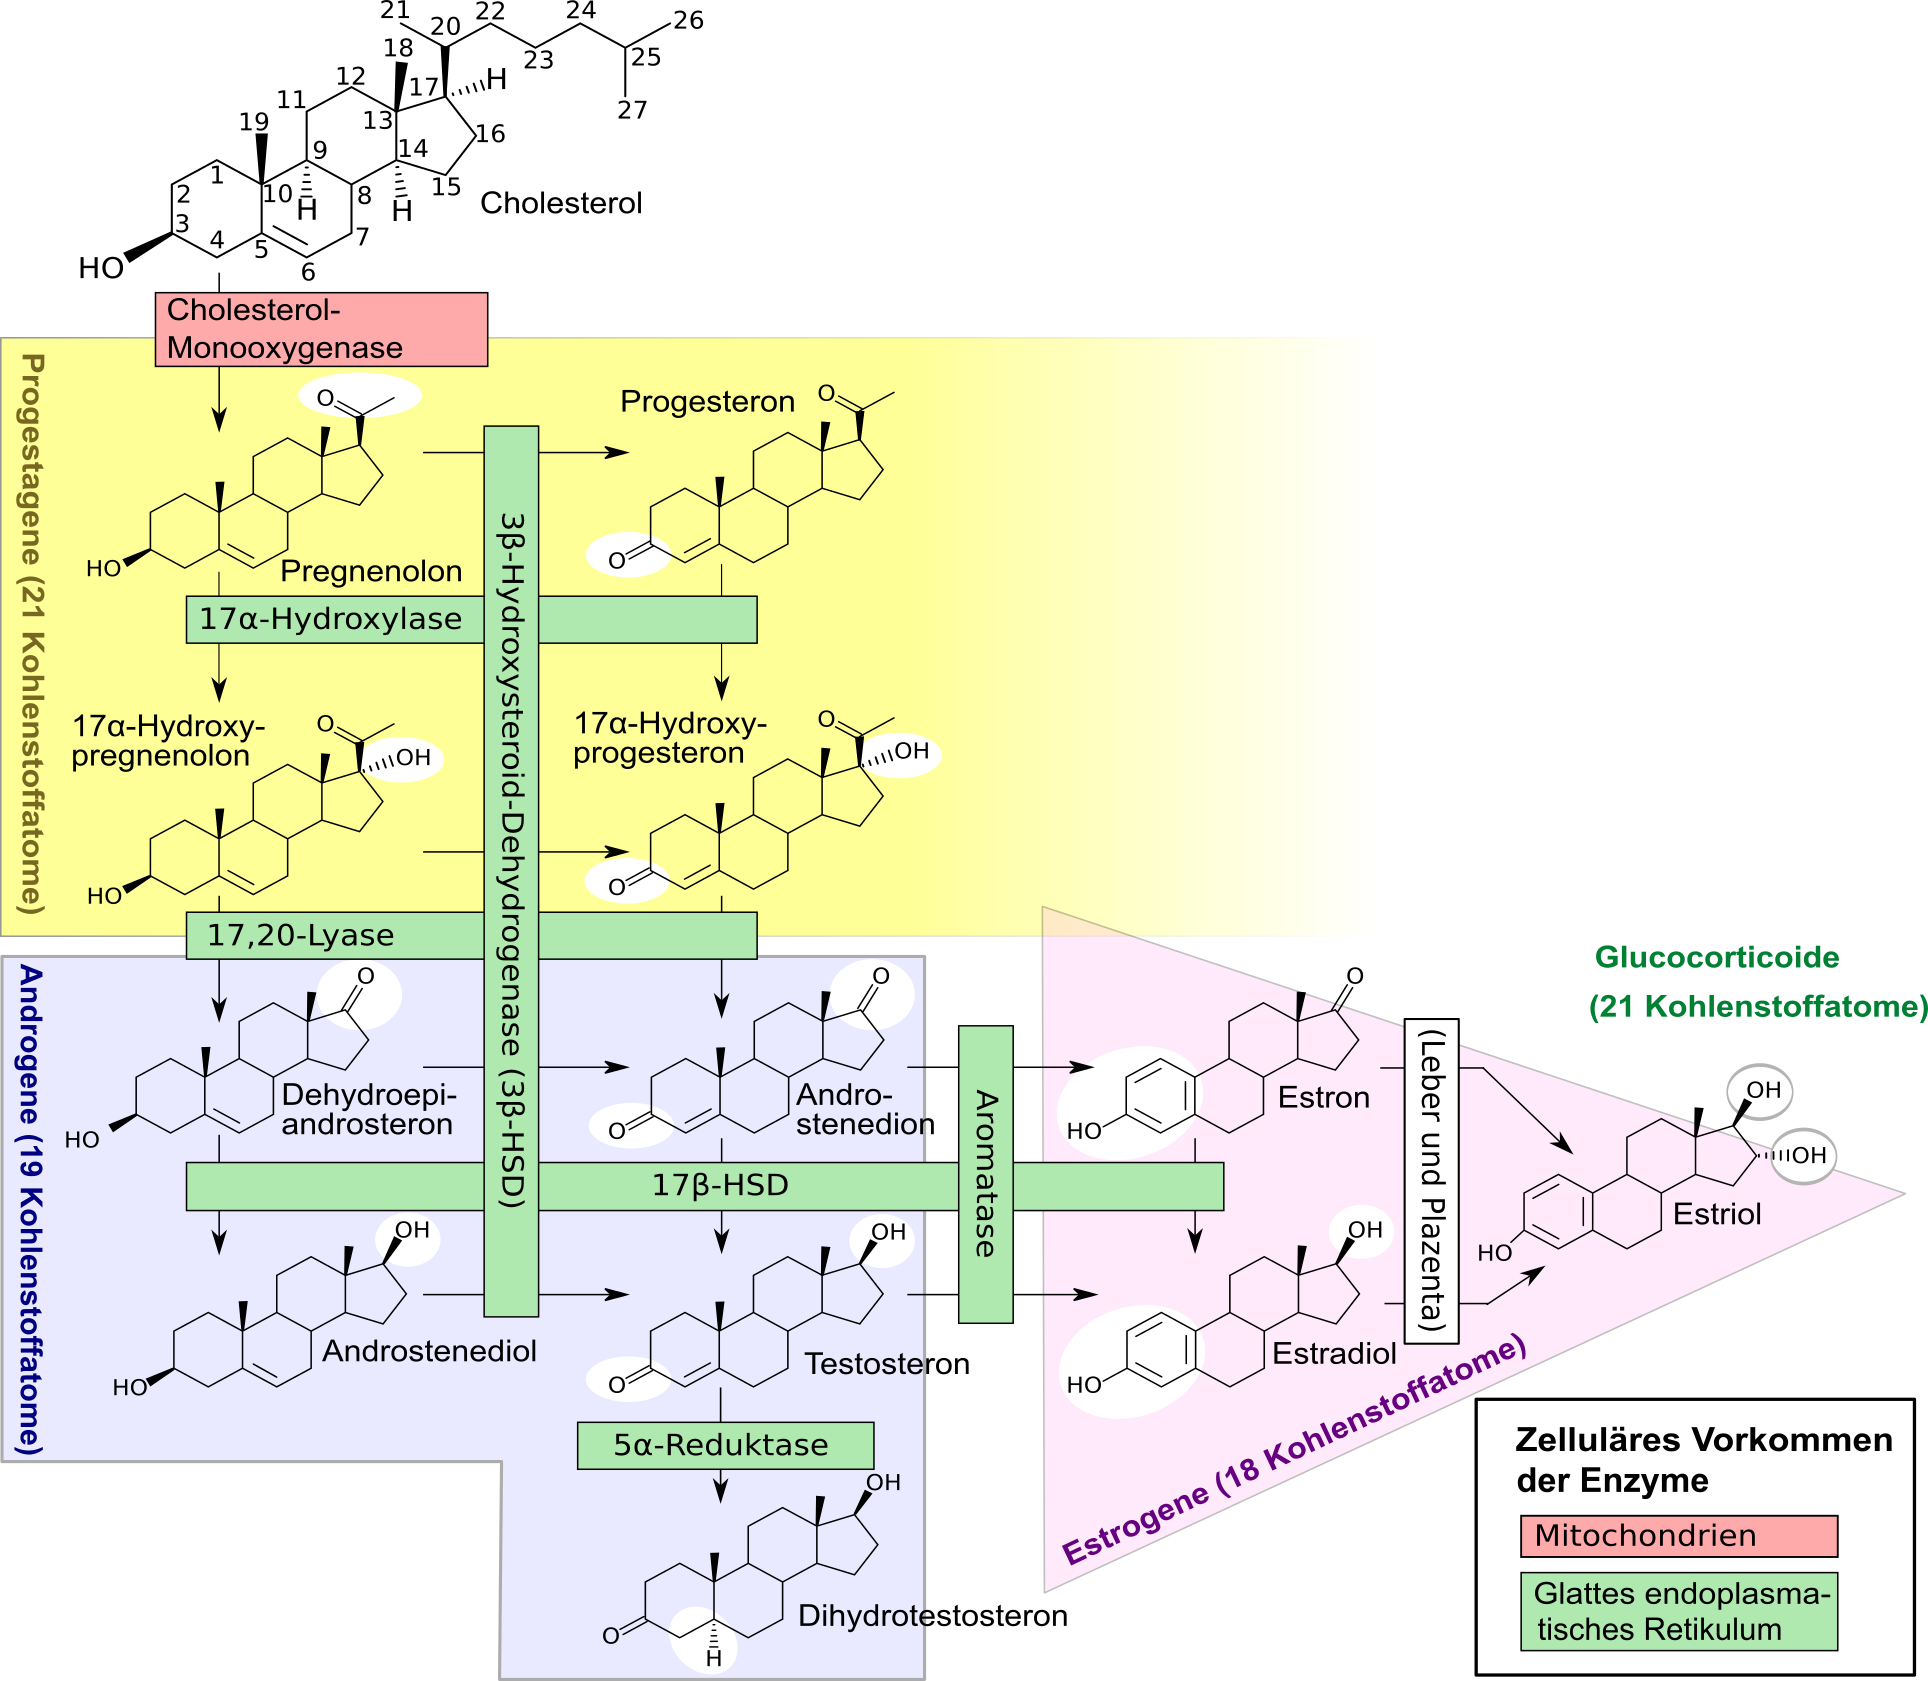
\includegraphics[width=\textwidth]{biosynthese_sexualhormone.png}
\end{center}



\end{column}

\pause

\begin{column}{6cm}

\pause

\begin{center}
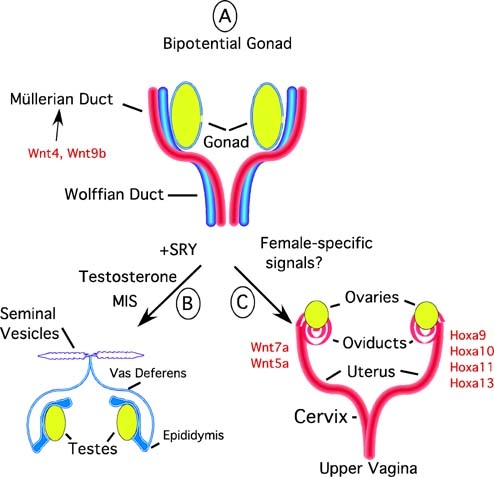
\includegraphics[width=\textwidth]{gonad_differentiation.jpg}
\end{center}


\end{column}



\end{columns}

    
\end{frame}


%5 Spermienbildung, Menstruation
% \begin{frame}{M11.10 Sexualentwicklung und Reproduktionsphysiologie I}

% \begin{columns}[c]

% \begin{column}{5cm}

% \begin{center}
%         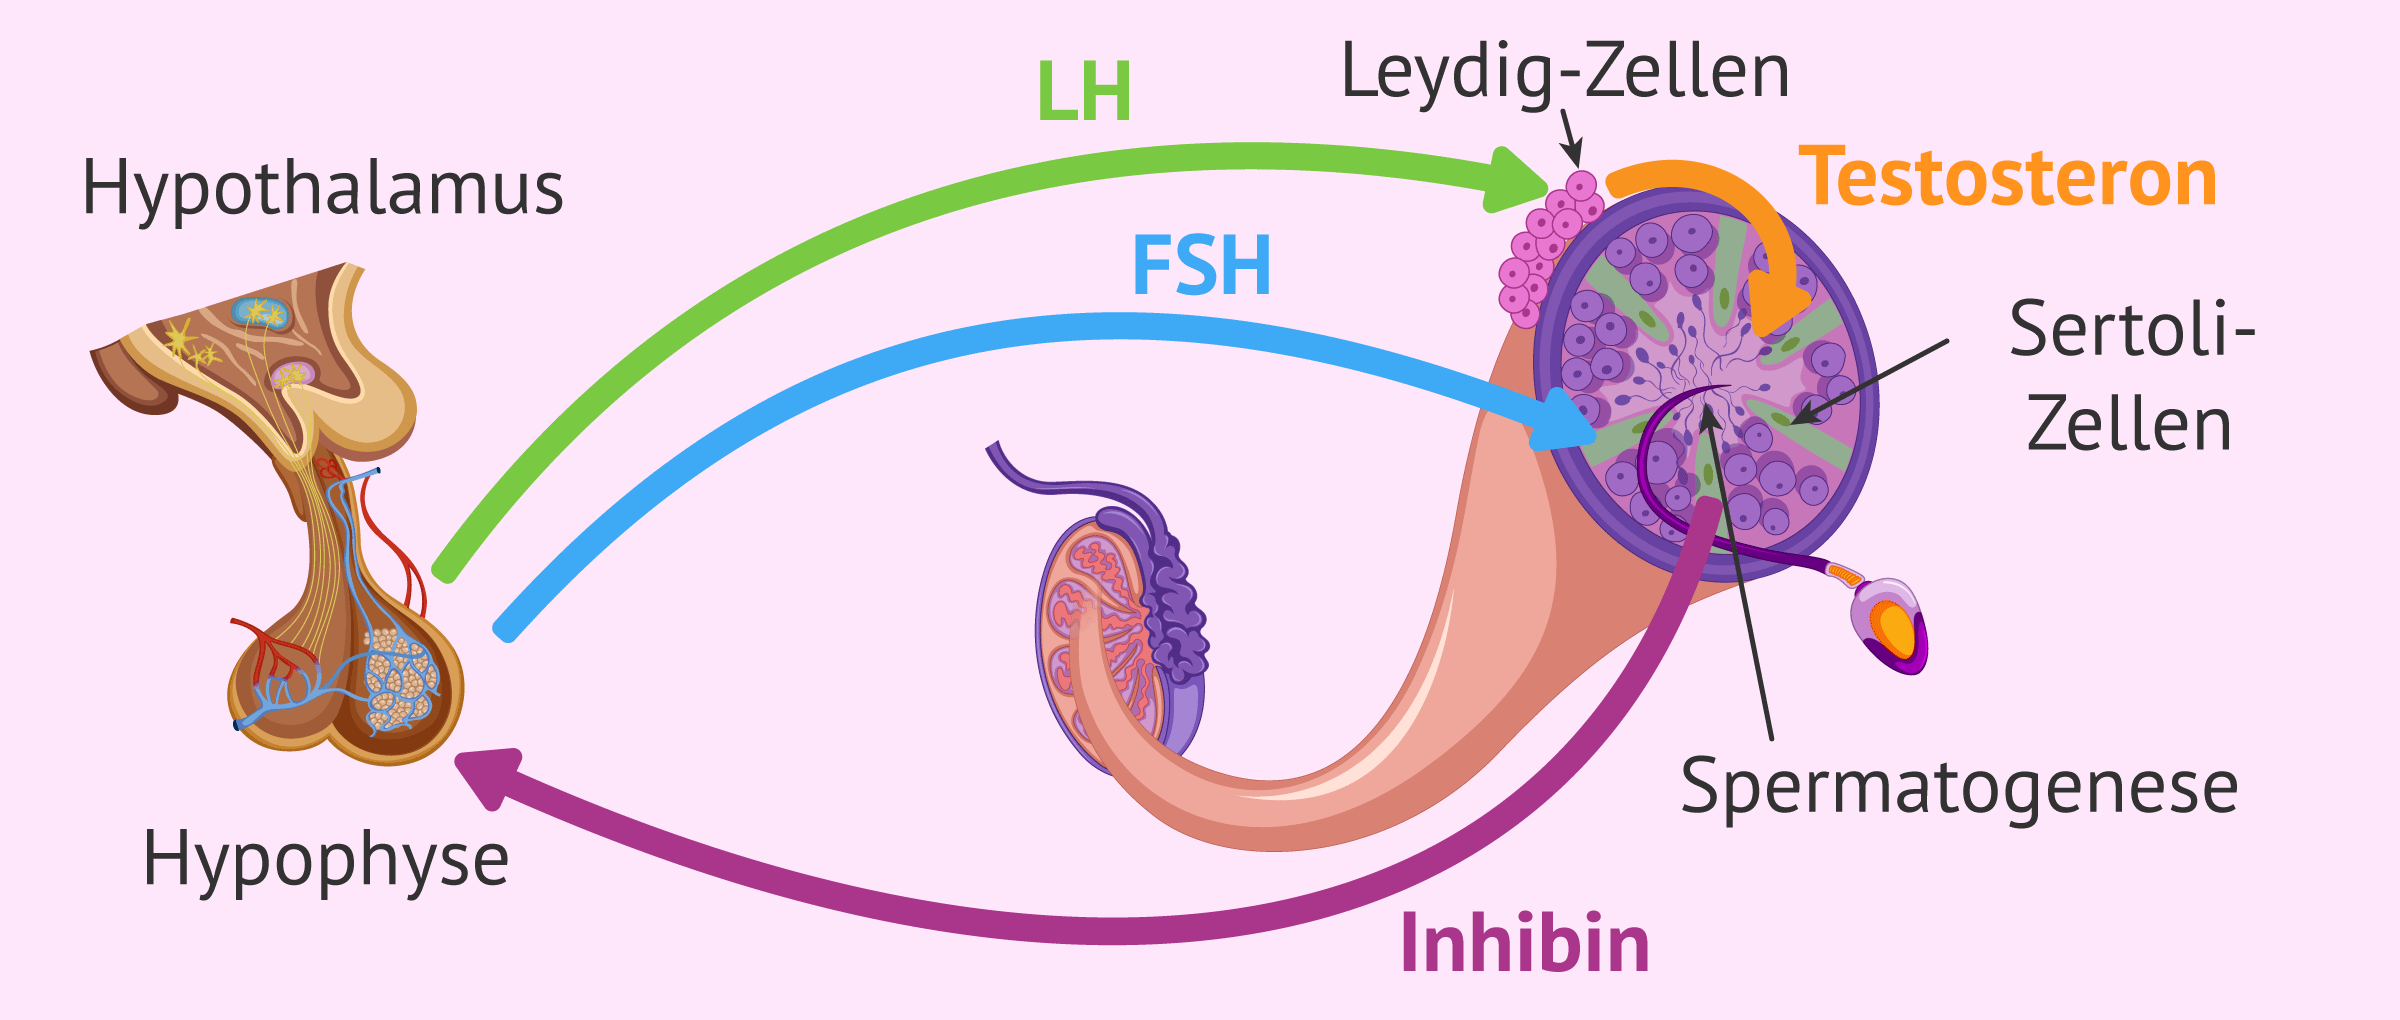
\includegraphics[width=\textwidth]{hormonelle-regulierung-spermatogenese.png}


%     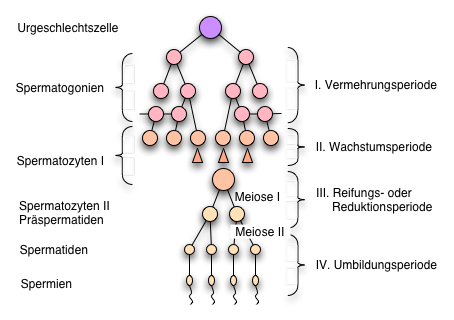
\includegraphics[width=\textwidth]{Spermatogenese.png}
    
% \end{center}



% \end{column}

% \pause

% \begin{column}{5cm}

% %% Zyklus

% \end{column}


% \end{columns}

% \end{frame}


%% Pubertät allgemein: 
% Menstruation: 199

% Testosteron 281


%%%%%%%%%%%%%%%%%%%%%%%%%%%%%%%%%%%%%%%%%%%%%%%%%%
%%%%%%%%%%%%%%%%%%%%%%%%%%%%%%%%%%%%%%%%%%%%%%%%%%
%%%%%%%%%%%%%%%%%%%%%%%%%%%%%%%%%%%%%%%%%%%%%%%%%%




% Hormonelle Veränderungen im Verlauf der Schwangerschaftbeschreiben und erklären
% die Entwicklung des Embryos und Fötus erklären
% die ”Fetoplazentare Einheit” und Funktion der Plazenta erläutern
% den Geburtsvorgang beschreiben und erklären
% die hormonelle Steuerung der Laktation erklären
% Erklären, wie ein Schwangerschaftstest funktioniert
% häufige Beschwerden und Komplikationen in der Schwangerschaft erklären


%% Verlauf von Schwangerschaft und Embryonalentwicklung
\begin{frame}{M11.10 Sexualentwicklung \& Reproduktionsphysiologie II: Schwangerschaft}

\begin{columns}[c]

\begin{column}{5cm}

\begin{center}
    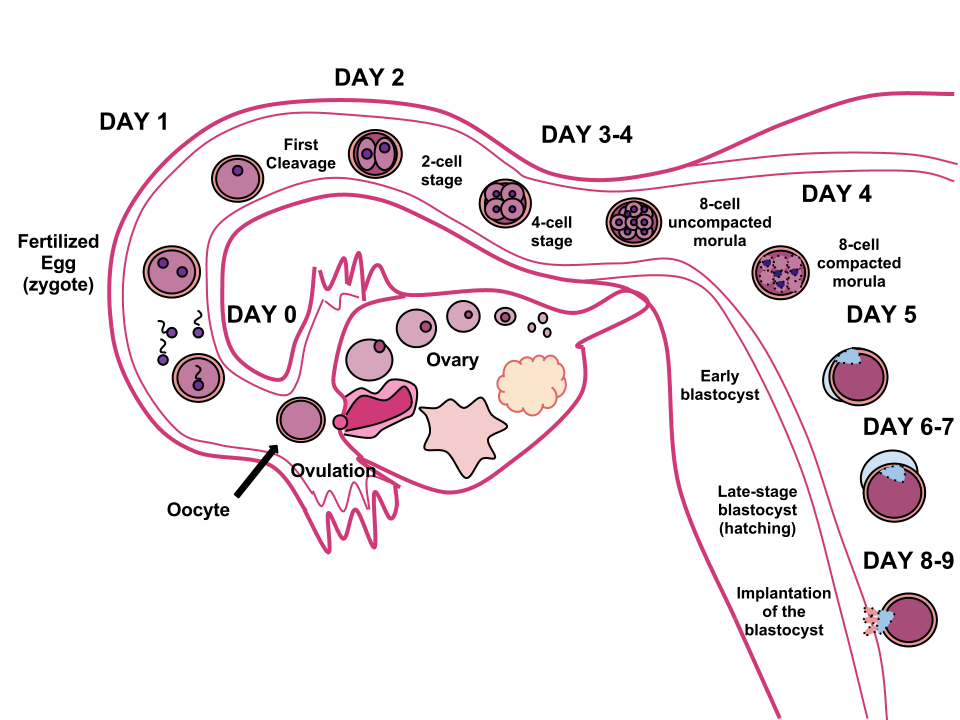
\includegraphics[width=\textwidth]{Human_Fertilization.png}
\end{center}

%% Hormone: HCG etc.
Embryo produziert humanes Choriongonadotropin (hCG). Ähnlich wie LH; fördert Progesteronbildung im Corpus luteum gravitas: Erhalt der Schwangerschaft 
\end{column}

\pause

\begin{column}{5cm}


\begin{center}
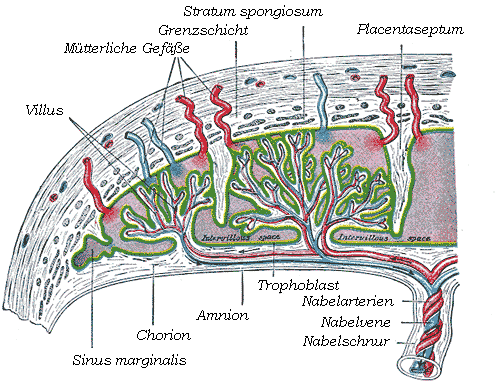
\includegraphics[width=0.8\textwidth]{Plazenta.png}    
\end{center}

% \small{Produktion von Östrogen und Progesteron ab SSW 9.}


\begin{center}
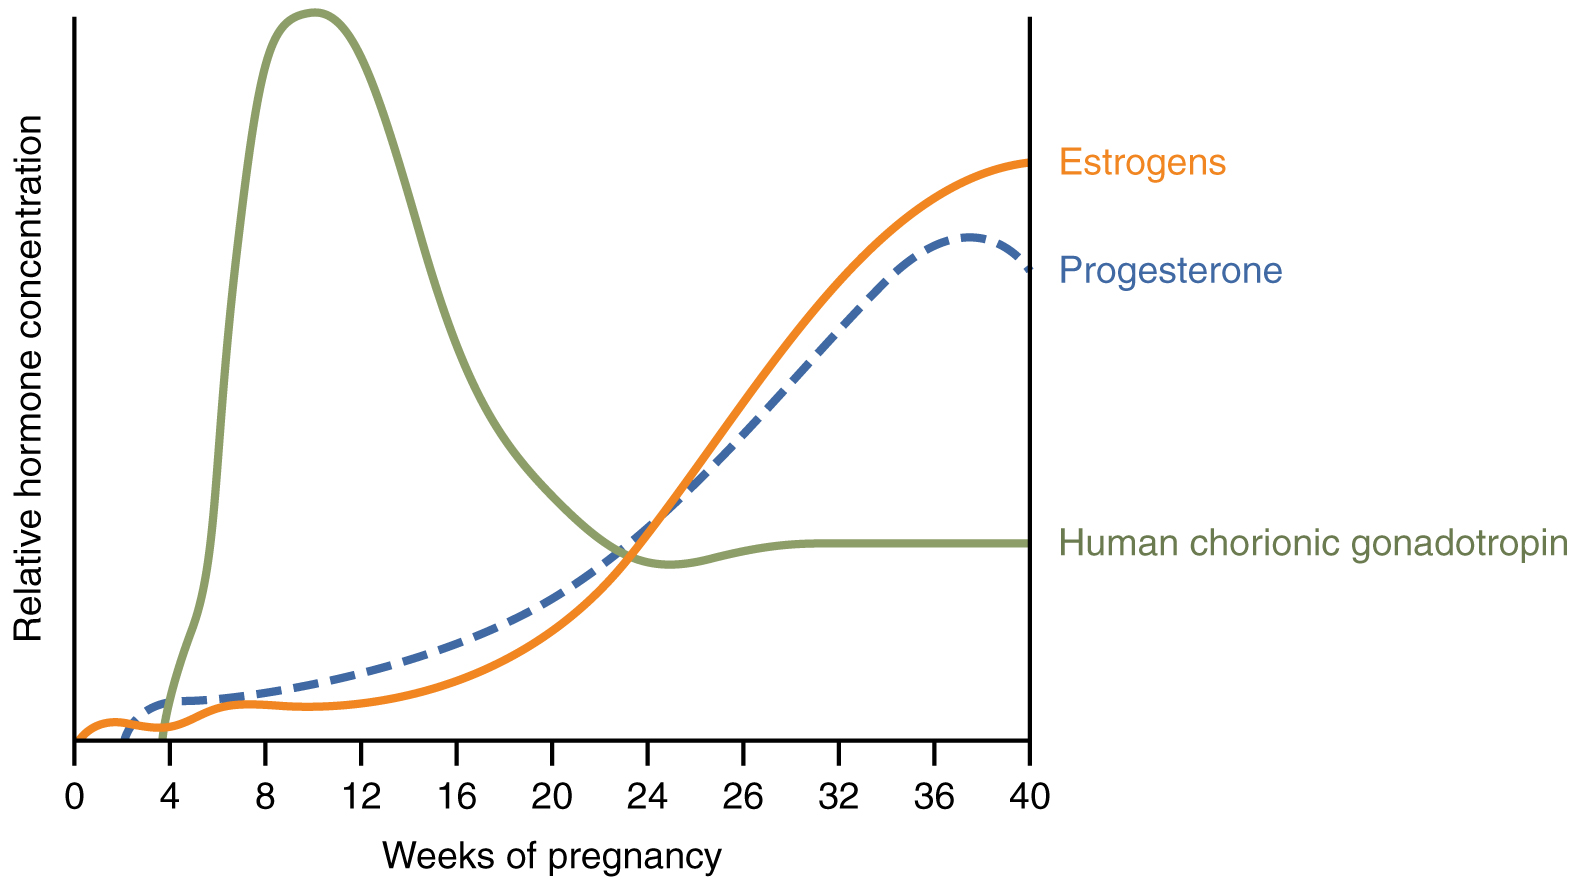
\includegraphics[width=\textwidth]{pregnancy_hormones.png}    
\end{center}



\end{column}

\end{columns}


\end{frame} 

\begin{frame}{M11.10 Sexualentwicklung \& Reproduktionsphysiologie II: Schwangerschaft}
    
    \begin{center}
        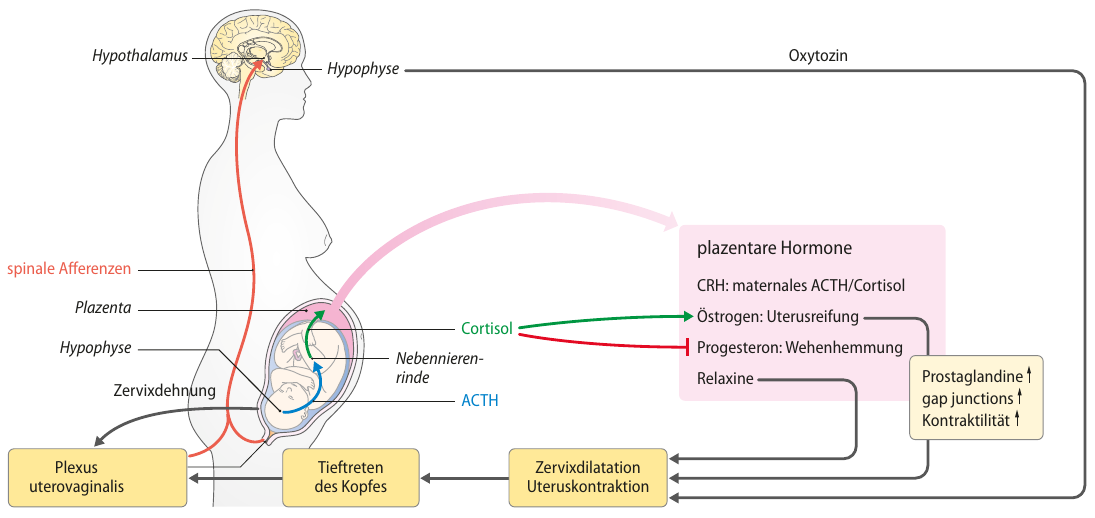
\includegraphics[width=\textwidth]{geburt_hormone.png}
    \end{center}
    
    \pause
    
    Laktation wird gesteuert durch Prolaktin aus der Adenohyphophyse (Milchbildung) und Oxytozin aus der Neurohypophyse (Milchfluss). Positive Rückkopplung durch Mechanorezeptoren an der Brustwarze. 
    
    
\end{frame}


%% IMPP Fragen zur Schwnagerschaft


%% Oxytocin: 477
\begin{frame}{IMPP Fragen}

\textbf{Welcher Neurotransmitter spielt bei der Förderung der Bindung zwischen Mutter und Kind am ehesten eine Rolle?
}\\[0.2 cm]

\begin{itemize}
\item[A.] Acetylcholin
\item[B.] Adrenalin
\item[C.] Dopamin
\item[D.] Noradrenalin
\item[E.] Oxytocin %% correct

\end{itemize}


\end{frame}



\begin{frame}{IMPP Fragen}

\textbf{Welcher Neurotransmitter spielt bei der Förderung der Bindung zwischen Mutter und Kind am ehesten eine Rolle?
}\\[0.2 cm]

\begin{itemize}
\item[A.] Acetylcholin
\item[B.] Adrenalin
\item[C.] Dopamin
\item[D.] Noradrenalin
\item[E.] \textcolor{blue}{Oxytocin} %% correct

\end{itemize}


\end{frame}




%% Fetales vs maternales Blut: 697 
\begin{frame}{IMPP Fragen}

\textbf{Welche Aussage zum arteriellen Blut eines Fetus in der 38. Schwangerschaftswoche trifft verglichen mit dem arteriellen Blut der Mutter am ehesten zu? }

\textbf{
In der Blutprobe des Fetus ist im Vergleich zur Blutprobe der Mutter
}\\[0.2 cm]

\begin{itemize}
\item[A.] der Anteil des Blutplasmas (am Volumen der Blutprobe) höher
\item[B.] der CO\textsubscript{2}-Partialdruck niedriger
\item[C.] der O\textsubscript{2}-Partialdruck niedriger %% correct
\item[D.] die Konzentration von IgM (Immunglobulin der Klasse M) im Blutplasma höher
\item[E.] die O\textsubscript{2}-Affinität niedriger, wenn bei gleichem pH-Wert untersucht wird 

\end{itemize}

    
\end{frame}


\begin{frame}{IMPP Fragen}

\textbf{Welche Aussage zum arteriellen Blut eines Fetus in der 38. Schwangerschaftswoche trifft verglichen mit dem arteriellen Blut der Mutter am ehesten zu? }

\textbf{
In der Blutprobe des Fetus ist im Vergleich zur Blutprobe der Mutter
}\\[0.2 cm]

\begin{itemize}
\item[A.] der Anteil des Blutplasmas (am Volumen der Blutprobe) höher
\item[B.] der CO\textsubscript{2}-Partialdruck niedriger
\item[C.] \textcolor{blue}{der O\textsubscript{2}-Partialdruck niedriger} %% correct
\item[D.] die Konzentration von IgM (Immunglobulin der Klasse M) im Blutplasma höher
\item[E.] die O\textsubscript{2}-Affinität niedriger, wenn bei gleichem pH-Wert untersucht wird 

\end{itemize}

\textcolor{blue}{Konkret:  O\textsubscript{2}-Partialdruck fötal: \(30\,mmHg\), elterlich: \(50\,mmHg\). \\ 
Damit der Stoffaustausch funktioniert, muss der  O\textsubscript{2}-Partialdruck im Fetus niedriger und der CO\textsubscript{2}-Partialdruck höher sein. 
    }
    
\end{frame}


%%%%%%%%%%%%%%%%%%%%%%%%%%%%%%%%%%%%%%%%%%%%%%%%%%
%%%%%%%%%%%%%%%%%%%%%%%%%%%%%%%%%%%%%%%%%%%%%%%%%%
%%%%%%%%%%%%%%%%%%%%%%%%%%%%%%%%%%%%%%%%%%%%%%%%%%

%% Vegetatives Nervensystem 1: Peripheres Nervensystem
\section{M11.11 Vegetatives Nervensystem 1: Peripheres Nervensystem }

%% Slides:


%% Slide 1: Komponenten des VNS
%% Sympathikus, Parasympathikus, enterisches Nervensystem  - sympa_parasympa.png
%% Emanuel slide 51 annotated: Sympathikus: fight or flight (ergotrop), parasympathikus: rest and digest  (trophotrop)

%% Verschaltung über Synspase, adners wie beim  

%%  Nebennierenmarkh
%% enterisches Nervensystem
%% Viszerale Afferenzen


%% SLide 2:

%% Übersicht to end all Übersichten: Emanuel Lecture 2 slide 6


%% Neurotransmitter und Rezeptoren
%% Peripheres NS: Verschaltung über Gaglion: Emanuel Slide 30
%% MUskarinerge Rezeptoren, Emanuel slide 35, anotate 
%% Adrenerge Rezepotiren, Emanuel slide 38
%% Cotransmitter: ATP; NO, Neuropeptide

%% Pharmacology: Indirekte, direkte Pharmakomimetika, Pharamtolytika



%% Sympathikus und Parasympathiku



%% IMPP: 



%% Verschaltung Sympathikus Parasympathikus: 286
%% Sympathikus Neurotransmiter: 587

%% Vielleicht Frage 115, 124 

%%%%%%%%%%%%%%%%%%%%%%%%%%%%%%%%%%%%%%%%%%%%%%%%%%
%%%%%%%%%%%%%%%%%%%%%%%%%%%%%%%%%%%%%%%%%%%%%%%%%%
%%%%%%%%%%%%%%%%%%%%%%%%%%%%%%%%%%%%%%%%%%%%%%%%%%
\section{M11.11 Vegetatives Nervensystem 2 Vegetative Zentren und Organregulation}

%% Vegetatives Nervensystem 2: Vegetative Zentren und Organregulation


%% Lernziele: 

% Welches sind die zentralen Komponenten des vegetaAven Nervensystems
% und wie steuern sie dessen FunkAon?
% •
% Limbisches System
% •
% •
% Hirnstamm
% •
% •
% Hypothalamus
% Medulla oblongata
% Rückenmark
% Wie steuert das VNS OrganfunkAonen?
% • Herz-Kreislauf-System
% • Magen-Darm-Trakt
% Wie verändern sich vegetaAve Reflexbahnen bei Querschnittlähmung?

 

%% Hierarchischer Aufbau des VNS - Slide 9
%% Lage und Anatomie des limbischen Systems . slide 14 mit Hypothalamus
%% Unterteilung des Hypothalamus? (S. 18)


%%% Read to p. 24

%%%%%%%%%%%%%%%%%%%%%%%%%%%%%%%%%%%%%%%%%%%%%%%% IMPP Fragen needed from here (search from 700)
%% Check special IMPP session


%% Herz

%% New 20: Pressorezeptoren
\begin{frame}{IMPP Fragen}


\textbf{ Welche Aussage zur Wirkung von Adrenalin/Noradrenalin am Herzen trifft im Allgemeinen zu?} \\[0.2 cm]

\begin{itemize}
\item[A.] 
\item[B.] 
\item[C.] 
\item[D.] 
\item[E.] 

\end{itemize}

    
\end{frame}


%% Harnblase: New 30

%%%%%%%%%%%%%%%%%%%%%%%%%%%%%%%%%%%%%%%%%%%%%%%%%%
%%%%%%%%%%%%%%%%%%%%%%%%%%%%%%%%%%%%%%%%%%%%%%%%%%
%%%%%%%%%%%%%%%%%%%%%%%%%%%%%%%%%%%%%%%%%%%%%%%%%%


%% Schlaf und EEG
\section{}

%% EEG 
%% Ableitung
%% Synchrone, asynchrone Aktivität

\begin{frame}{M11.11 ZNS 2: Schlaf und EEG} 

\begin{columns}[c]

\begin{column}{5cm}

\begin{center}
    
    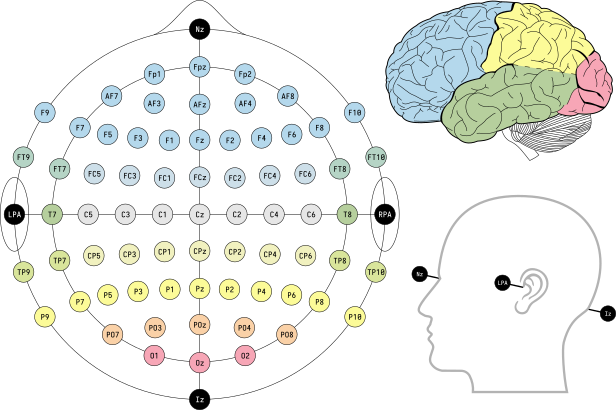
\includegraphics[width=\textwidth]{EEG_10-10_system.png}
    
    
    \end{center}
    
    $\,$\\
    
    \begin{center}
        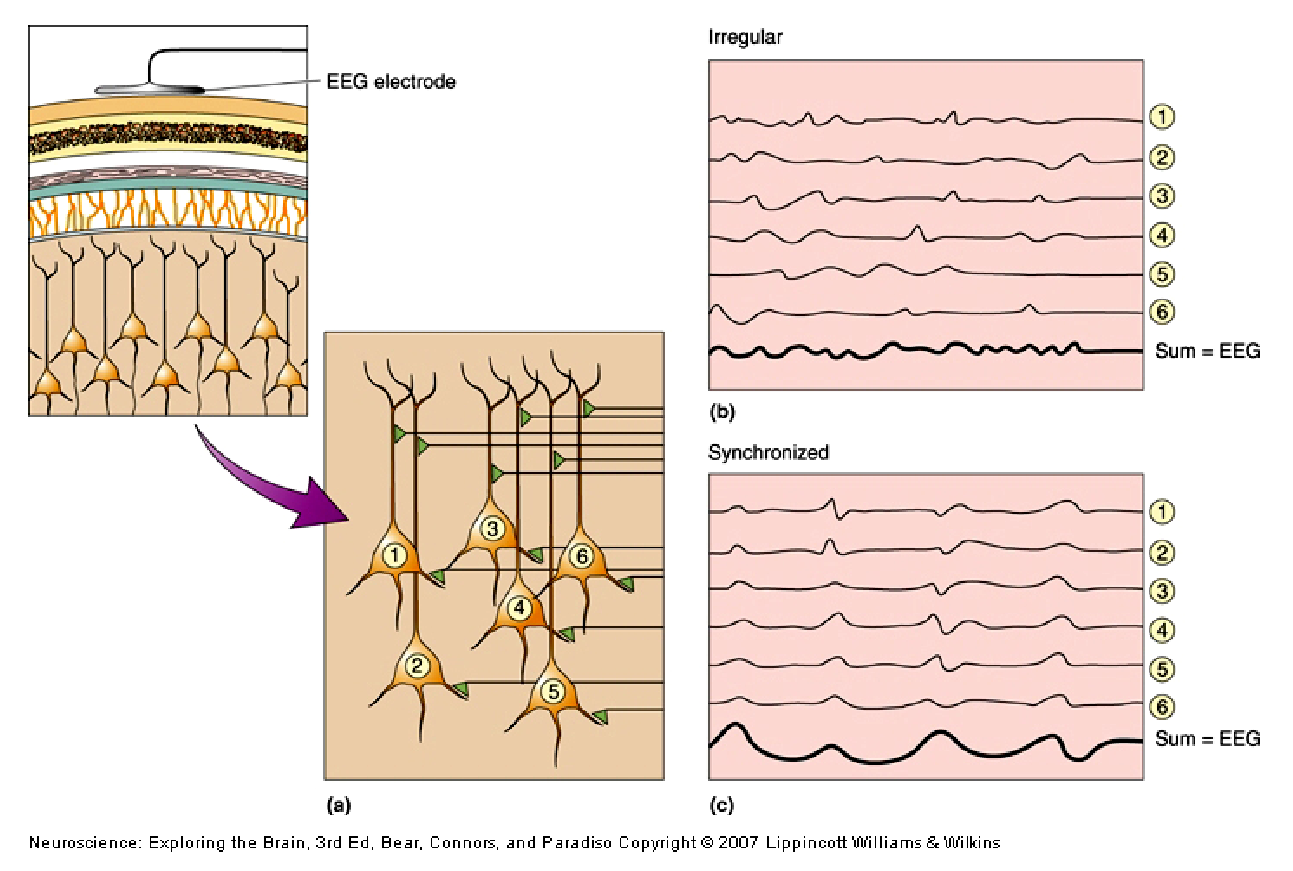
\includegraphics[width=\textwidth]{EEG_synchrony..png}

\end{center}

\end{column}

\begin{column}{6cm}

EEG misst Summe aus vielen synchronen EPSPs.   \\
Amplitude: \\ \(50-100\,\mu V\) (Hintergrund-EEG), \\ \(1-15\mu V\) (evozierte Potentiale) \\
Räumliche Auflösung: cm-Bereich \\
Zeitliche Auflösung: \(0.5-30\,\)Hz \\ \pause
Bei neurologische Krankheiten oft atypisches EEG, z.B. Epilepsie 


\begin{center}
    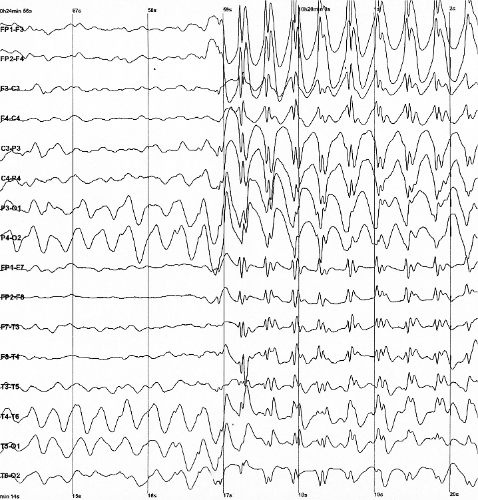
\includegraphics[width=0.6\textwidth]{Spike-waves.png}
\end{center}


\end{column}


\end{columns}

\end{frame}




%% Schlaf und Epilepsie
%% ARAS; Übergang zwischen Schlafphasen, EEG bei Schlaf 
\begin{frame}{M11.11 ZNS 2: Schlaf und EEG}
    
    %% both formatio reticularis slides
    \begin{columns}[c]
    \begin{column}{6cm}
    
    \begin{center}
        \includegraphics<1>[width=\textwidth]{formatio_reticularis_1.pdf}
        \includegraphics<2->[width=\textwidth]{formatio_reticularis_2.pdf}
    \end{center}
    
    \pause
    
    
    \end{column}
    
    \begin{column}{5cm}
    
    \pause
    
    \begin{block}{Schlaf EEG}
    
    \begin{center}
        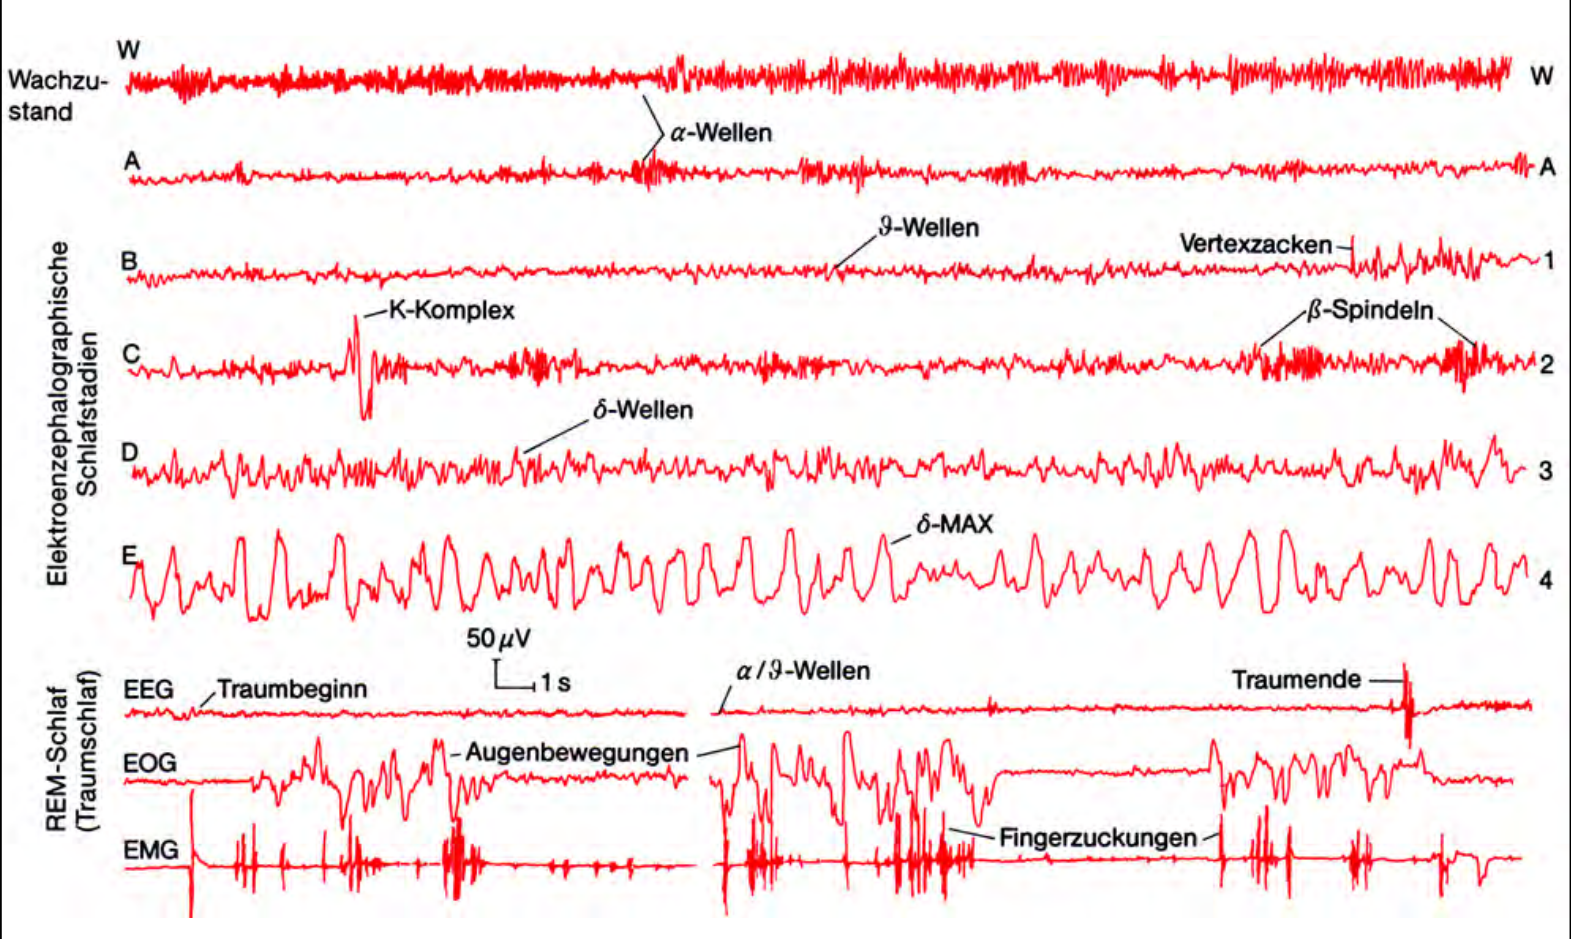
\includegraphics[width=\textwidth]{schlaf_eeg.png}
    \end{center}
    
    \end{block}
    
    \end{column}
    
    
    \end{columns}
    
    
    \pause

\begin{block}{Kontrolle der Schlafphasen}
\begin{columns}[c]
\begin{column}{3cm}
    \begin{center}
        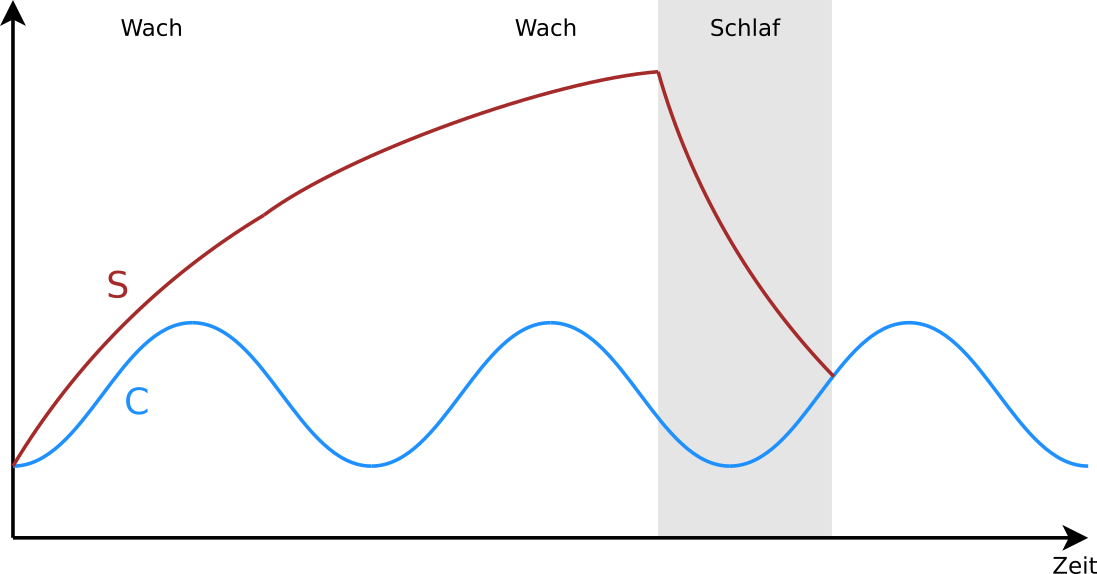
\includegraphics[width=\textwidth]{Zwei-prozess-2.png}
    \end{center}
    
    \end{column}
    
    \begin{column}{8cm}
    Homöostatischer Faktor: Adenosoin  \\
    Rhytmischer Faktor: Circadianer Rhythmus \\
    Übergang zwischen REM und non-REM Schlaf wird im Pons kontrolliert. 


    
    \end{column}
    
    \end{columns}
    



    
    
    \end{block}
    
\end{frame}



%% EEG allgemein - 112
\begin{frame}{IMPP Fragen}

\textbf{
Welche Aussage zum (in üblicher Weise abgeleiteten) EEG eines Gesunden trifft am ehesten zu?
} \\[0.2 cm]

\begin{itemize}
\item[A.] Die räumliche Auflösung des EEG ermöglicht die Lokalisation einzelner kortikaler Neurone
\item[B.] Im Wachzustand haben die Potenzialschwankungen im EEG eine durchschnittliche Amplitude von \(5-10\,mV\)
\item[C.] \(\beta\)-Wellen haben durchschnittlich höhere Amplituden als \(\alpha\)-Wellen
\item[D.] Wellen mit einer Amplitude von über \(100\,\mu V\) lassen sich im EEG nur bei wachen Personen ableiten
\item[E.] Zum Auftreten von \(\alpha\)-Wellen im EEG trägt die synchrone Aktivität thalamokortikaler Verbindungen bei. %% correct

\end{itemize}

\end{frame}


\begin{frame}{IMPP Fragen}

\textbf{
Welche Aussage zum (in üblicher Weise abgeleiteten) EEG eines Gesunden trifft am ehesten zu?
} \\[0.2 cm]

\begin{itemize}
\item[A.] Die räumliche Auflösung des EEG ermöglicht die Lokalisation einzelner kortikaler Neurone
\item[B.] Im Wachzustand haben die Potenzialschwankungen im EEG eine durchschnittliche Amplitude von \(5-10\,mV\)
\item[C.] \(\beta\)-Wellen haben durchschnittlich höhere Amplituden als \(\alpha\)-Wellen
\item[D.] Wellen mit einer Amplitude von über \(100\,\mu V\) lassen sich im EEG nur bei wachen Personen ableiten
\item[E.] \textcolor{blue}{Zum Auftreten von \(\alpha\)-Wellen im EEG trägt die synchrone Aktivität thalamokortikaler Verbindungen bei.} %% correct

\end{itemize}

\end{frame}



%% Schlaf

\begin{frame}{IMPP Fragen}

\textbf{Sie sitzen vor dem Computer im Schlaflabor und analysieren ein EEG eines Patienten. Dabei beobachten Sie überwiegend Wellen im Frequenzbereich zwischen 8 und 12\,Hz. }
\textbf{Welcher Bewusstseinsgrad ist für den Patienten am ehesten zutreffend?} \\[0.2 cm]

\begin{itemize}
\item[A.] Aktivation
\item[B.] entspannter Wachzustand
\item[C.] Ermüdung
\item[D.] hohe Aufmerksamkeit
\item[E.] Tiefschlaf
\end{itemize}

\end{frame}


\begin{frame}{IMPP Fragen}

\textbf{Sie sitzen vor dem Computer im Schlaflabor und analysieren ein EEG eines Patienten. Dabei beobachten Sie überwiegend Wellen im Frequenzbereich zwischen 8 und 12\,Hz. }
\textbf{Welcher Bewusstseinsgrad ist für den Patienten am ehesten zutreffend?} \\[0.2 cm]

\begin{itemize}
\item[A.] Aktivation
\item[B.] \textcolor{blue}{entspannter Wachzustand  - \(\alpha\)-Wellen}  
\item[C.] Ermüdung
\item[D.] hohe Aufmerksamkeit
\item[E.] Tiefschlaf
\end{itemize}

\end{frame}



%%%%%%%%%%%%%%%%%%%%%%%%%%%%%%%%%%%%%%%%%%%%%%%%%%
%%%%%%%%%%%%%%%%%%%%%%%%%%%%%%%%%%%%%%%%%%%%%%%%%%
%%%%%%%%%%%%%%%%%%%%%%%%%%%%%%%%%%%%%%%%%%%%%%%%%%


%% Lernen und Plastizität

%% Slide 1
%%  Arten von Gedächtnis, Arten des Lernens: Zeit (+ Aufmerksamkeit), assoziativ, nicht-assoziativ, Modelllernen
\begin{frame}{M11.11 ZNS 3: Lernen und Plastizität} 

\end{frame}



%% Slide 2

%% Hebbsche Synapse, LTP + Molekular
\begin{frame}{M11.11 ZNS 3: Lernen und Plastizität} 

\end{frame}


%% IMPP Fragen

%% Allgemein: Implizites Lernen: 358
\begin{frame}{IMPP Fragen}

\textbf{Welche der Aussagen über das implizite Lernen bzw. Gedächtnis trifft am ehesten zu?} \\[0.2 cm]

\begin{itemize}
\item[A.] Bei beidseitiger Schädigung de Hippocampus ist implizites Lernen nicht mehr möglich.
\item[B.] Bei Patienten mit anterograder Amnesie ist implizites Lernen nicht mehr möglich.
\item[C.] Beim impliziten Lernen ist vor allem die mediale Temporallappenregion aktiv.
\item[D.] Das prozedurale Gedächtnis speichert typischerweise Fakten.
\item[E.] Implizite Lernvorgänge beruhen u.a. auf Plastizität in Basalganglien und Zerebellum %% correct

\end{itemize}

\end{frame}


\begin{frame}{IMPP Fragen}

\textbf{Welche der Aussagen über das implizite Lernen bzw. Gedächtnis trifft am ehesten zu?} \\[0.2 cm]

\begin{itemize}
\item[A.] Bei beidseitiger Schädigung de Hippocampus ist implizites Lernen nicht mehr möglich.
\item[B.] Bei Patienten mit anterograder Amnesie ist implizites Lernen nicht mehr möglich.
\item[C.] Beim impliziten Lernen ist vor allem die mediale Temporallappenregion aktiv.
\item[D.] Das prozedurale Gedächtnis speichert typischerweise Fakten.
\item[E.] \textcolor{blue}{Implizite Lernvorgänge beruhen u.a. auf Plastizität in Basalganglien und Zerebellum} %% correct

\end{itemize}

\end{frame}



%% Mehr LTP 
%% 123

\begin{frame}{IMPP Fragen}

\textbf{Die Langzeitspeicherung von Informationen im menschlichen Gehirn erfolgt durch plastische Veränderungen an zentralen Synapsen.}

\textbf{Welcher der folgenden Prozesse ist typischerweise an der Auslösung der Langzeitpotenzierung (LTP) der synaptischen Übertragung in exzitatorischen Synapsen beteiligt? } \\[0.2 cm]

\begin{itemize}
\item[A.] Aufhebung des Mg\textsuperscript{2+}-Blocks der NMDA-Rezeptoren durch Aktivierung von AMPA-Rezeptoren
\item[B.] erniedrigte Ca\textsuperscript{2+}-Permeabilität von AMPA-Rezeptoren in der postsynaptischen Membran
\item[C.] Hyperpolarisation der postsynaptischen Membran durch retrograde Ausbreitung somatischer Aktionspotentiale
\item[D.] reduzierte Offenwahrscheinlichkeit präsynaptischer Calciumkanäle vom P/Q Typ
\item[E.] vermehrte Endozytose von AMPA-Rezeptoren an der postsynaptischen Membran

\end{itemize}

\end{frame}


\begin{frame}{IMPP Fragen}

\textbf{Die Langzeitspeicherung von Informationen im menschlichen Gehirn erfolgt durch plastische Veränderungen an zentralen Synapsen.}

\textbf{Welcher der folgenden Prozesse ist typischerweise an der Auslösung der Langzeitpotenzierung (LTP) der synaptischen Übertragung in exzitatorischen Synapsen beteiligt? } \\[0.2 cm]

\begin{itemize}
\item[A.] \textcolor{blue}{Aufhebung des Mg\textsuperscript{2+}-Blocks der NMDA-Rezeptoren durch Aktivierung von AMPA-Rezeptoren}
\item[B.] erniedrigte Ca\textsuperscript{2+}-Permeabilität von AMPA-Rezeptoren in der postsynaptischen Membran
\item[C.] Hyperpolarisation der postsynaptischen Membran durch retrograde Ausbreitung somatischer Aktionspotentiale
\item[D.] reduzierte Offenwahrscheinlichkeit präsynaptischer Calciumkanäle vom P/Q Typ
\item[E.] vermehrte Endozytose von AMPA-Rezeptoren an der postsynaptischen Membran

\end{itemize}

\end{frame}



\begin{frame}{IMPP Fragen}

\textbf{Welcher der folgenden Prozesse ist typischerweise an der Auslösung der Langzeitpotenzierung (LTP) der synaptischen Übertragung in exzitatorischen Synapsen beteiligt? } \\[0.2 cm]

\begin{itemize}
\item[A.] \textcolor{blue}{Aufhebung des Mg\textsuperscript{2+}-Blocks der NMDA-Rezeptoren durch Aktivierung von AMPA-Rezeptoren}
\end{itemize}



\begin{center}
    \includegraphics<1>[width=0.8\textwidth]{LTP1_AMPAR.png}
    \includegraphics<2>[width=0.8\textwidth]{LTP2_depol.png}
        \includegraphics<3>[width=0.8\textwidth]{LTP3_NMDAR.png}
        \includegraphics<4>[width=0.8\textwidth]{LTP4_Ca.png}
\end{center}

\end{frame}



%%%%%%%%%%%%%%%%%%%%%%%%%%%%%%%%%%%%%%%%%%%%%%%%%%
%%%%%%%%%%%%%%%%%%%%%%%%%%%%%%%%%%%%%%%%%%%%%%%%%%
%%%%%%%%%%%%%%%%%%%%%%%%%%%%%%%%%%%%%%%%%%%%%%%%%%


%% Motorik 1 
\begin{frame}{M11.12 Motorik 1: Grundlagen und Reflexe} 


\begin{columns}[c]

\begin{column}{5cm}
\begin{block}{Muskelspindel}


Misst Dehnung (Ia, II) \\
% \(\gamma\)-Faser ermöglicht Sensitivität \\
Parallel zum Muskel \\

\begin{center}
    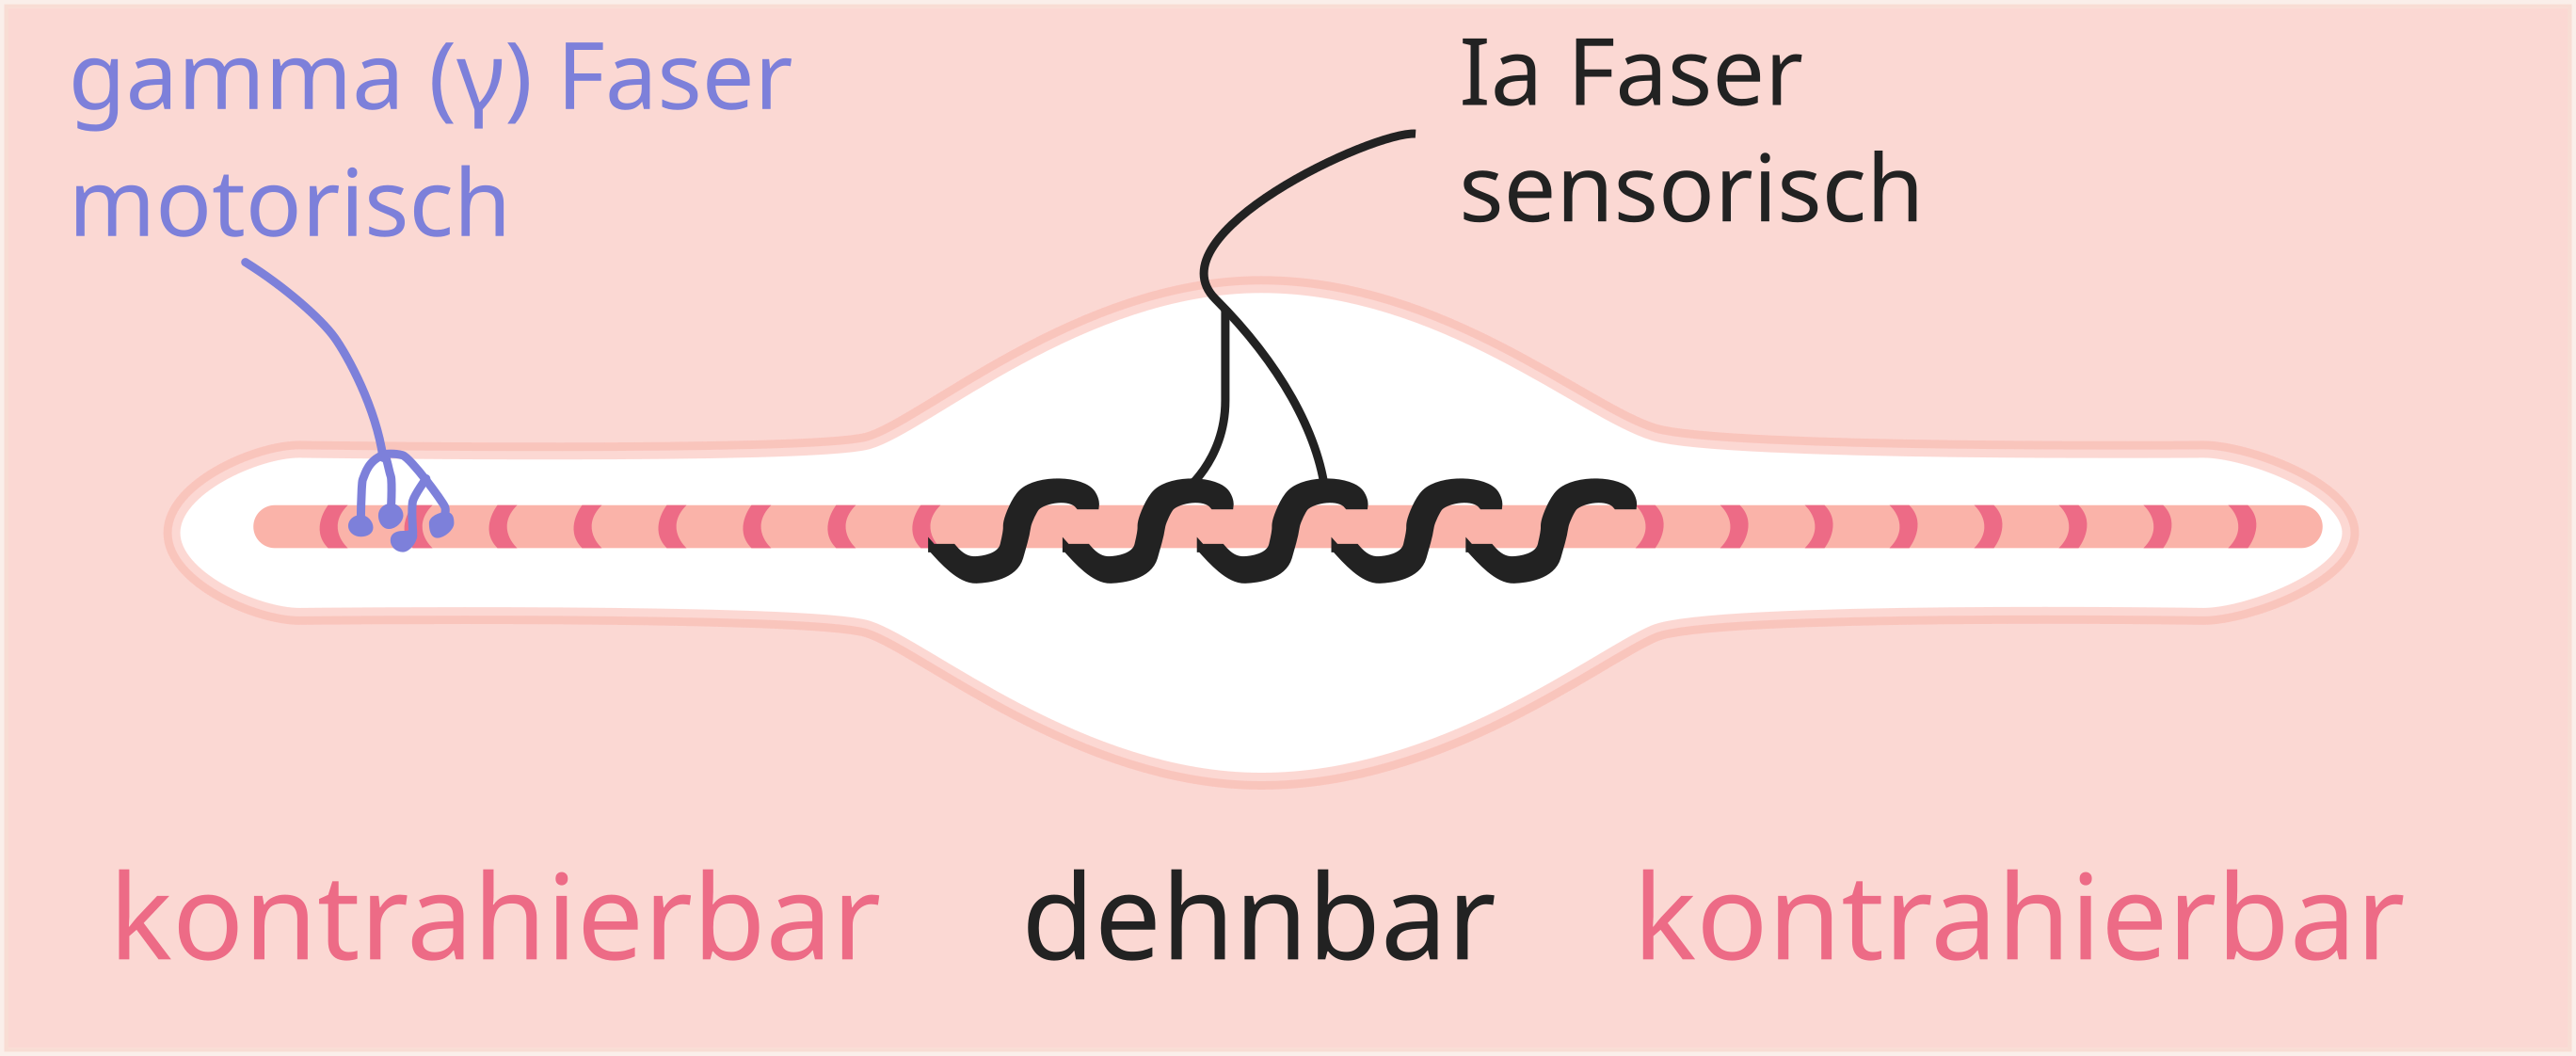
\includegraphics[width=\textwidth]{MuscleSpindle.png}
\end{center}

\end{block}

\begin{block}{Golgi-Sehnen-Organ}

Misst Spannung (Ib)\\
Seriell zum Muskel


\begin{center}
    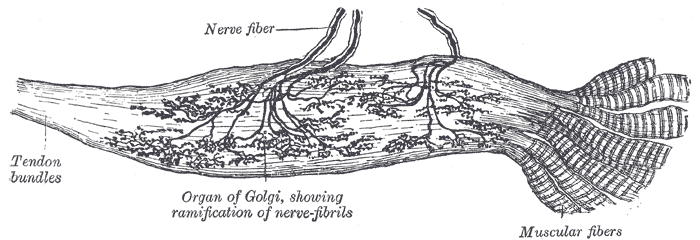
\includegraphics[width=0.8\textwidth]{Gray938.png}
\end{center}


\end{block}
\end{column}

\pause

\begin{column}{5cm}

\textbf{Vestibularsystem}: Gleichgewicht, Haltung  \\


\textbf{Cerebellum}: Kontrolle, Koordination, Feinabstimmung \\

\pause

\begin{center}
    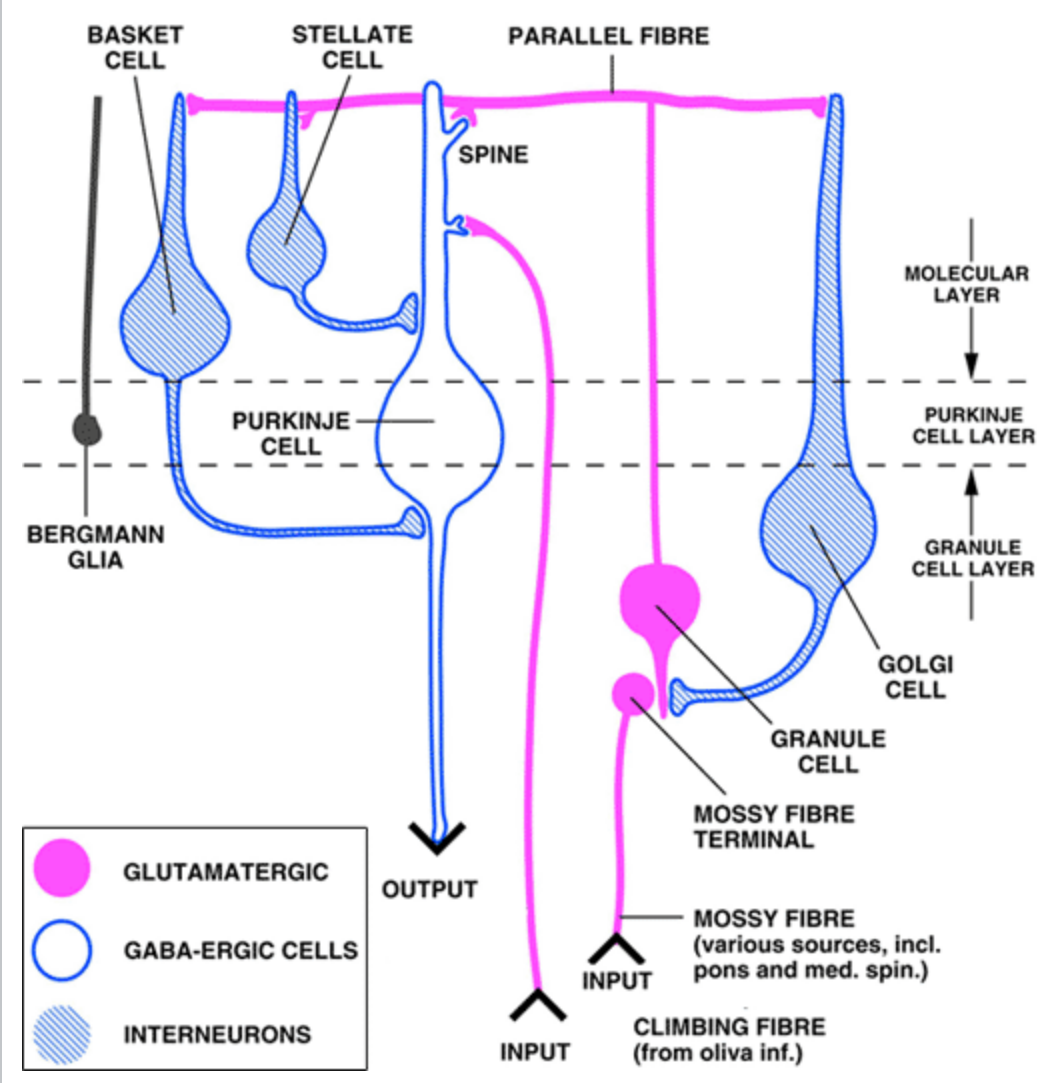
\includegraphics[width=\textwidth]{cerebellum_layers.png}
\end{center}

\end{column}


\end{columns}

%% Sesnsorische Organe in Muskeln

%%  Vestibulärsystem, Cerebellu

\end{frame}



% \begin{frame}{M11.12 Motorik 1: Grundlagen und Reflexe} 

% %% Rückenmark
% %%  Reflexbogen

% \begin{columns}[c]
% \begin{column}{5cm}
% Rückenmark \\

% \begin{center}
%     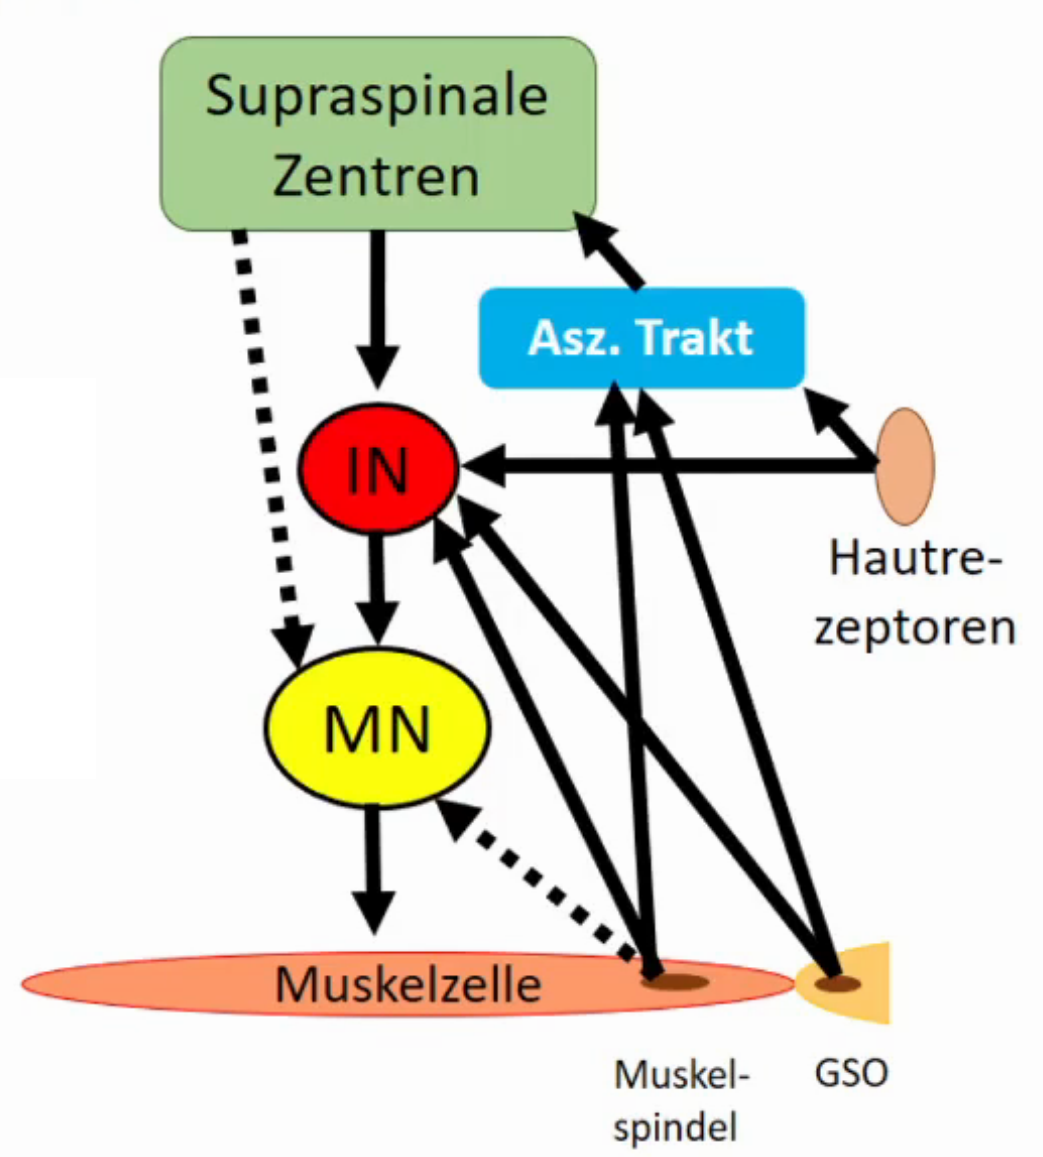
\includegraphics[width=\textwidth]{rueckenmark_orga.png}
% \end{center}

% \pause



% \end{column}

% \begin{column}{5cm}

% Reflexbogen \\

% \begin{center}
%     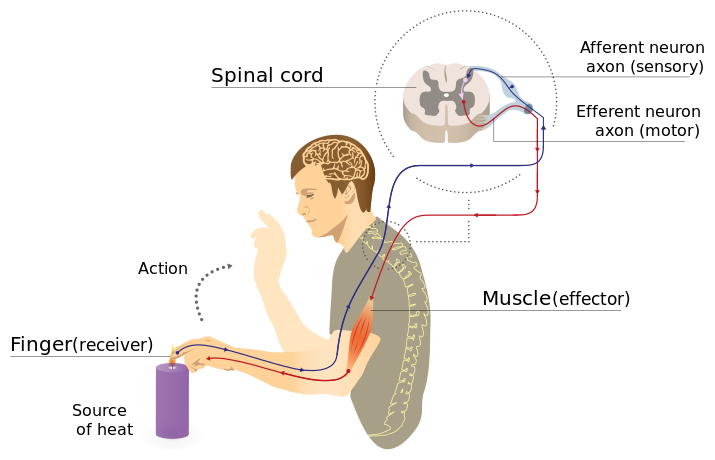
\includegraphics[width=\textwidth]{reflex_arc.png}
% \end{center}

% Eigenreflexe, Frendreflexe3 Jul 2022



% \end{column}


% \end{columns}


% %% Eigen-, Fremdreflexe




% \end{frame}



%% 416 - Muskelspindeln
%% 191 - Reflexe


%%%%%%%%%%%%%%%%%%%%%%%%%%%%%%%%%%%%%%%%%%%%%%%%%%
%%%%%%%%%%%%%%%%%%%%%%%%%%%%%%%%%%%%%%%%%%%%%%%%%%
%%%%%%%%%%%%%%%%%%%%%%%%%%%%%%%%%%%%%%%%%%%%%%%%%%


%% Motorik 2

\begin{frame}{M11.12 Motorik 2: Willkürbewegungen} 

%% Basalganglien

Basalganglien kontrollieren Bewegungsabläufe, indem sie gewünschte Bewegungen fördern (Go-Weg) und unerwünschte Bewegungen unterdrücken (No-Go-Weg); wichtig dabei Dopamin aus der SnC

\begin{center}
    \includegraphics<1>[width=0.7\textwidth]{Basalganglien_direkt.png}
    \includegraphics<2>[width=0.7\textwidth]{Basalganglien_direkt_indirekt.png}
    \includegraphics<3>[width=0.7\textwidth]{Basalganglien_all.png}
\end{center}


\end{frame}

%% Motorkortex, Hirnstamm, Deszendierende Bahnen
\begin{frame}{M11.12 Motorik 2: Willkürbewegungen} 

\begin{columns}[c]

\begin{column}{5cm}
Motorischer Kortex:

\begin{center}
    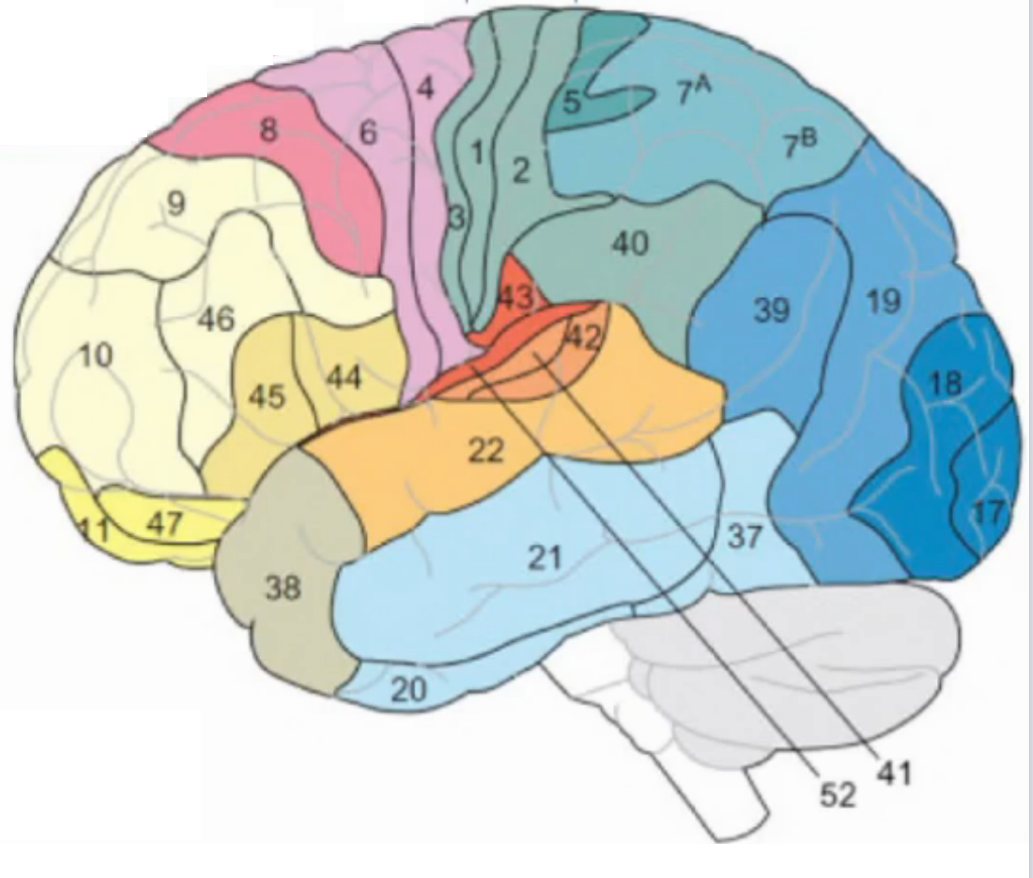
\includegraphics[width=\textwidth]{cortex.png}
\end{center}


Prämotorischer Kortex (Area 6): Erstellung Bewegungsprogramm \\
Primärmotorischer Kortex (M1, Area 4): Durchführung Bewegungsprogramm \\ 
Frontales Augenfeld (Area 8): Willkürbewegung der Augen \\

\end{column}

\begin{column}{5cm}



\end{column}


\end{columns}

\end{frame}


%% 178 - Parkinson Fall

%% 136

%% Pyramidenbahn? 967


\end{document}
 
%%% Frequently used snippets

%% \begin{columns}[c]

%% \begin{column}{5cm}
%% \end{column}

%% \begin{column}{5cm}
%% \end{column}


%% \end{columns}




%% IMPP Frage

% \textbf{Frage} \\[0.2 cm]

% \begin{itemize}
% \item[A.]
% \item[B.]
% \item[C.]
% \item[D.]
% \item[E.]

% \end{itemize}